%% 
%% Copyright 2007, 2008, 2009 Elsevier Ltd
%% 
%% This file is part of the 'Elsarticle Bundle'.
%% ---------------------------------------------
%% 
%% It may be distributed under the conditions of the LaTeX Project Public
%% License, either version 1.2 of this license or (at your option) any
%% later version.  The latest version of this license is in
%%    http://www.latex-project.org/lppl.txt
%% and version 1.2 or later is part of all distributions of LaTeX
%% version 1999/12/01 or later.
%% 
%% The list of all files belonging to the 'Elsarticle Bundle' is
%% given in the file `manifest.txt'.
%% 
%% Template article for Elsevier's document class `elsarticle'
%% with harvard style bibliographic references
%% SP 2008/03/01

\documentclass[preprint,12pt,authoryear]{elsarticle}

%% Use the option review to obtain double line spacing
%% \documentclass[authoryear,preprint,review,12pt]{elsarticle}

%% Use the options 1p,twocolumn; 3p; 3p,twocolumn; 5p; or 5p,twocolumn
%% for a journal layout:
%% \documentclass[final,1p,times,authoryear]{elsarticle}
%% \documentclass[final,1p,times,twocolumn,authoryear]{elsarticle}
%% \documentclass[final,3p,times,authoryear]{elsarticle}
%% \documentclass[final,3p,times,twocolumn,authoryear]{elsarticle}
%% \documentclass[final,5p,times,authoryear]{elsarticle}
%% \documentclass[final,5p,times,twocolumn,authoryear]{elsarticle}

%% For including figures, graphicx.sty has been loaded in
%% elsarticle.cls. If you prefer to use the old commands
%% please give \usepackage{epsfig}

%% The amssymb package provides various useful mathematical symbols
\usepackage{amssymb}
\usepackage{amsmath}
\usepackage{color, soul}
\usepackage{url}
%% The amsthm package provides extended theorem environments
%% \usepackage{amsthm}

%% The lineno packages adds line numbers. Start line numbering with
%% \begin{linenumbers}, end it with \end{linenumbers}. Or switch it on
%% for the whole article with \linenumbers.
\usepackage{lineno}

%% Block of code for fixing corresponding author bug 
%% in elsarticle template... Don't really understand it
\makeatletter
\def\@author#1{\g@addto@macro\elsauthors{\normalsize%
    \def\baselinestretch{1}%
    \upshape\authorsep#1\unskip\textsuperscript{%
      \ifx\@fnmark\@empty\else\unskip\sep\@fnmark\let\sep=,\fi
      \ifx\@corref\@empty\else\unskip\sep\@corref\let\sep=,\fi
      }%
    \def\authorsep{\unskip,\space}%
    \global\let\@fnmark\@empty
    \global\let\@corref\@empty  %% Added
    \global\let\sep\@empty}%
    \@eadauthor={#1}
}
\makeatother
%% End block of weird code


%% Command for bold Greek symbols
\newcommand{\mitbf}[1]{\hbox{\mathversion{bold}$#1$}}

\journal{Earth and Planetary Science Letters}

\begin{document}

\begin{frontmatter}

%% Title, authors and addresses

%% use the tnoteref command within \title for footnotes;
%% use the tnotetext command for theassociated footnote;
%% use the fnref command within \author or \address for footnotes;
%% use the fntext command for theassociated footnote;
%% use the corref command within \author for corresponding author footnotes;
%% use the cortext command for theassociated footnote;
%% use the ead command for the email address,
%% and the form \ead[url] for the home page:
%% \title{Title\tnoteref{label1}}
%% \tnotetext[label1]{}
%% \author{Name\corref{cor1}\fnref{label2}}
%% \ead{email address}
%% \ead[url]{home page}
%% \fntext[label2]{}
%% \cortext[cor1]{}
%% \address{Address\fnref{label3}}
%% \fntext[label3]{}

\title{Bayesian inversion for paleomagnetic reconstruction and plate kinematics}

%% use optional labels to link authors explicitly to addresses:
%% \author[label1,label2]{}
%% \address[label1]{}
%% \address[label2]{}

\author{Ian Rose\corref{cor1}\fnref{ref1}}
\author{Bruce Buffett\fnref{ref1}}
\author{N.L. Swanson-Hysell\fnref{ref1}}

\fntext[ref1]{University of California, Berkeley}
\cortext[cor1]{Corresponding author, \url{ian.rose@berkeley.edu}}

\address{}

\begin{abstract}
%% Text of abstract

\end{abstract}

\begin{keyword}
%% keywords here, in the form: keyword \sep keyword

%% PACS codes here, in the form: \PACS code \sep code

%% MSC codes here, in the form: \MSC code \sep code
%% or \MSC[2008] code \sep code (2000 is the default)

\end{keyword}

\end{frontmatter}

\linenumbers

%% main text
\section{Introduction}
\label{sec:introduction}

Plate tectonics is the motion of near-rigid blocks of lithosphere across the surface of Earth, 
separated by narrow regions of deformation in spreading centers, transform faults, and subduction zones.
The overall rigidity of plate motions means that the motion of a great majority of Earth's surface
can be described by a set of Euler poles which determine the position and magnitude of the rotation axis for a
given plate \citep[cf.][]{cox2009plate}. The motion of individual points on a plate undergoing
a rigid rotation is described by small circles.

Euler poles are ubiquitous in describing current plate motions 
\citep[e.g.][]{demets1990current, argus2011geologically} due to their simplicity and compactness.
Furthermore, there are good reasons to think that plate motions remain constant, or approximately
so, over millions to tens of millions of years. This is most dramatically seen in the shape
of oceanic fracture zones and in hotspot tracks across the lithosphere. These features
form gently curving arcs over large portions of Earth's surface which are well described by small
circles, consistent with finite Euler rotations of the plate for an extended period of time.
As such, the combination of an Euler pole plus a time interval through which it rotates 
(often called a ``stage pole'') is a convenient description of plate motions through Earth history.

The stage pole description of plate motions is therefore a convenient way of reconstructing
plate tectonic history, and is widely used in both continental reconstruction 
\citep[e.g.][]{boyden2011next} and in geodynamical
modeling \citep[e.g.][]{mcnamara2005thermochemical, bull2014effect, rudolph2014history}.
Most reconstructions of plate motions rely heavily on fitting Euler pole rotations
to oceanic fracture zones, hotspot tracks, seafloor magnetic isochrons,
and, to a lesser extent, paleomagnetic data \citep{muller1993revised, seton2012global}.
However, as we look further back in Earth history, the records on which these
plate tectonic reconstructions rely largely disappear due to the continual
subduction of oceanic lithosphere. Before $\sim$200 Ma there is no oceanic record,
and the paleomagnetic record from continental rocks is all that remains.

It is more challenging to reconstruct past plate motions from the paleomagnetic
record for a number of reasons, including 
(1) the data is usually sparser and with larger uncertainties,
(2) traditional paleomagnetic analysis has no way of constraining paleolongitude, and
(3) many paleomagnetic poles have poor age control.

\citet{gordon1984paleomagnetic} noted that apparent polar wander paths (APWPs) have 
arcing trajectories similar to fracture zones and hotspot tracks, which is
to be expected if similar tectonic processes are responsible for creating them.
They therefore suggested fitting small circles to paleomagnetic poles tracks,
which would furnish Euler poles for the plate in question for that time period.
This model for understaning APWPs, called paleomagnetic Euler pole (PEP) analysis,
 had the attractive feature of providing a complete description of the plate motion, 
including paleolongitudinal changes and speeds. 
However, it had the drawback of being somewhat difficult to calculate,
uncertainties in the fit were not easily computed, 
and it did not incorporate age uncertainties. 
A rigorous treatment of the uncertainties requires significant computational effort.
With a few exceptions \citep{beck1989paleomagnetism, tarling1996palaeomagnetic, bryan1986rotation, beck2003absolute, smirnov2010co} 
PEP analysis has not seen wide adoption.

Herein we extend paleomagnetic Euler pole analysis by placing it within
a Bayesian statistical framework, and demonstrate how to invert for PEPs
using Markov Chain Monte Carlo (MCMC) methods. This framework has the advantage
of naturally incorporating uncertainties in the paleomagnetic pole positions,
as well as widely disparate age uncertainties that commonly occur in APWPs.
The resulting stage poles for which we invert is not a single answer, but is instead
a distribution of possible answers, furnishing uncertainties as part of the solution process.

The paper is organized as follow. In Section~\ref{sec:apwp} we review different
approaches for interpreting APWPs. In Section~\ref{sec:bayesian_inversion} we
describe the formalism of Bayesian inversions and Markov Chain Monte Carlo methods.
In Section~\ref{sec:model} we describe the statistical model which we will be inverting.
In Section~\ref{sec:example_inversion} we demonstrate the inversion on several
synthetic data sets. In Sections~\ref{sec:australia} and~\ref{sec:keweenawan}
we show examples using real paleomagnetic data from Australia and Laurentia,
including interpretations of plate speeds.

\section{Interpretation of APW paths}
\label{sec:apwp}

\subsection{Latitudinal drift}
\subsection{Running means and spline fits}
\subsection{Paleomagnetic Euler poles}
\citet{gordon1984paleomagnetic}

\section{Bayesian inversion}
\label{sec:bayesian_inversion}
\subsection{Bayes theorem}

\begin{equation}
P\left(A \vert B \right) = \frac{ P \left(B \vert A \right) P \left(A\right) }{P \left(B\right)}
\label{eq:bayes}
\end{equation}
It is often unnecessary to calculate the denominator of Equation~\eqref{eq:bayes}, leaving
\begin{equation}
P\left(A \vert B \right) \propto P \left(B \vert A \right) P \left(A\right) 
\label{eq:propbayes}
\end{equation}
\subsection{Distributions on a sphere}

In order to proceed with a Bayesian description of the problem, every parameter
in the model should be described by some statistical distribution that determines
the probability that the parameter takes a specific value.
In addition to several more familiar 1D distributions (such as uniform or normal distributions)
we will also need to describe the statistics of points on a sphere, which we 
review here.


\subsubsection{Uniform distribution}
\begin{figure*}
\includegraphics[width=0.9\textwidth]{figures/cartoon/uniform.pdf}
\caption{Probability density for the uniform spherical distribution, as well as samples drawn from that distribution, plotted with an orthographic projection.}
\label{fig:uniform}
\end{figure*}

The simplest probability distribution on a sphere is the spherical uniform distribution, shown in Figure~\ref{fig:uniform}.
It has a probability density given by
\begin{equation}
  \rho(\phi, \psi) = \frac{1}{4 \pi},
\end{equation}
where $\rho$ is the probability density, $\phi$ is the longitude, and $\psi$ is the latitude.
Most non-uniform distributions on a sphere reduce to the uniform distribution in some limit.
We will use this distribution when we want to specify an uninformative prior for directional parameters.

\subsubsection{Fisher distribution}
The Fisher distribution (also called the von Mises-Fisher distribution) is the analogue
of a 2D normal distribution on a sphere. It is shown in Figure~\ref{fig:fisher}.
The probability density for a unit vector $\hat{\mathbf{x}}$ is given by
\begin{equation}
  \begin{aligned}
  \rho(\psi, \phi) 
  &= \frac{1}{C_F} \exp \left( \kappa_F \hat{\mathbf{x}}^T \hat{\mitbf{\mu}} \right) \\
  &= \frac{1}{C_F} \exp \left( \kappa_F \cos \theta \right),
  \end{aligned}
\end{equation}
where $C_F$ is a normalization factor, $\kappa$ is the concentration of the distribution, and
$\hat{\mitbf{\mu}}$ the unit vector of the mean of the distribution. It can be alternatively
parameterized using $\theta$, which is the angle between $\hat{\mathbf{x}}$ and $\hat{\mitbf{\mu}}$.
The normalization factor is given by 
\begin{equation}
  C_F = \frac{\kappa_F}{4 \pi \sinh{\kappa}}.
\end{equation}
The position and uncertainty of most paleomagnetic poles are represented by Fisher distributions,
and so we will use it to calculate the likelihood function of the model.

\begin{figure*}
\includegraphics[width=0.9\textwidth]{figures/cartoon/fisher.pdf}
\caption{Probability density for a Fisher distribution, as well as samples drawn from that distribution, plotted with an orthographic projection. The center of the distribution is at $30^\circ$N, $30^\circ$E, and the concentration parameter $\kappa=20$.}
\label{fig:fisher}
\end{figure*}

\subsubsection{Watson girdle distribution}
\begin{equation}
  \begin{aligned}
  \rho(\psi, \phi) 
  &= \frac{1}{C_W} \exp \left( \kappa_W (\hat{\mathbf{x}}^T \hat{\mitbf{\mu}})^2 \right) \\
  &= \frac{1}{C_W} \exp \left( \kappa_W \cos^2 \theta \right)
  \end{aligned}
\end{equation}
\begin{equation}
  C_W = \left[ {}_1 F_1 \left( \frac{1}{2}, \frac{3}{2}, \kappa_W \right) \right]^{-1}
\end{equation}

\begin{figure*}
\includegraphics[width=0.9\textwidth]{figures/cartoon/watson.pdf}
\caption{Probability density for the Watson girdle distribution, as well as samples drawn from that distribution, plotted with an Orthographic projection. The pole of symmetry is at $70^\circ$N, $90^\circ$E, and the concentration parameter $\kappa=-5$.}
\label{fig:watson}
\end{figure*}
\subsection{Markov chain Monte Carlo methods}

\section{A model for PEP inversion}
\label{sec:model}
\subsection{Forward model}
The forward model for PEP analysis is essentially unchanged from that of \citet{gordon1984paleomagnetic}.
We describe plate motions (and hence paleomagnetic pole motions) with a series of Euler poles.
Each Euler pole has three parameters for which we are inverting (a latitude, a longitude and a rotation rate).

We furthermore need a set of changepoints, which denote the ages where we transition from 
one Euler pole to the next (the cusps, or ``hairpins'' of \citet{irving1972hairpins}).

Finally, we need a starting position on the globe, which, in practice, can be sampled
from the Fisher distribution of the oldest paleomagnetic pole in the dataset.
The starting point contributes two parameters (a latitude and a longitude).

All together, this means that the number of parameters for which we are inverting is given by
\begin{equation}
\begin{aligned}
N &= 3 n_e + (n_e -1) + 2 \\
 &= 4 n_e + 1
\end{aligned}
\label{eq:n_parameters}
\end{equation}

For each Euler pole $\mitbf{\omega}$ the velocity $\mathbf{v}$ of a point 
$\mathbf{p}$ on the surface of the globe is given by
\begin{equation}
\mathbf{v} = \mitbf{\omega} \times \mathbf{p}.
\label{eq:rigid_rotation}
\end{equation}
Finite rotations can be performed by constructing Euler angle rotation matrices \citep[cf.][]{goldstein1965classical}. 


\subsection{Choice of priors}

\subsection{Likelihood}

\subsection{Model selection}

\section{Example inversions}
\label{sec:example_inversion}


\subsection{One stage pole}
\begin{figure*}
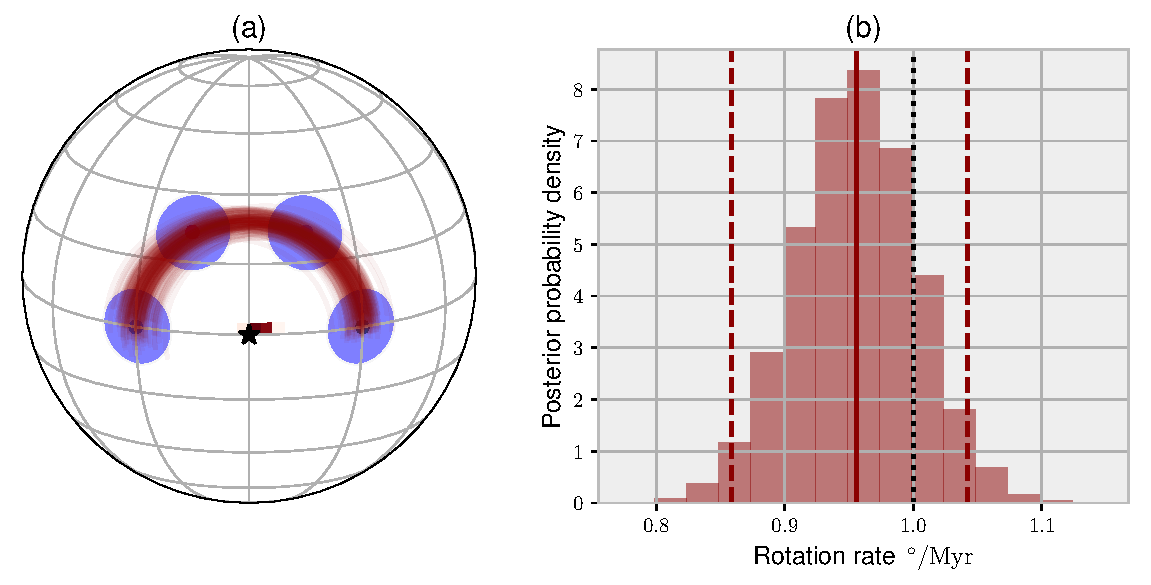
\includegraphics[width=0.9\textwidth]{figures/synthetic/one_euler_pole.pdf}
\caption{Inversion for a single paleomagnetic Euler pole (PEP). (a) Four paleomagnetic poles are generated by a $180^\circ$ rotation about an Euler pole at $0^\circ$N, $0^\circ$E over 30 Myr, for a rotation rate of $6^\circ$/Myr. The red distribution is the probability density function recovered by MCMC inversion, and the red lines are a sampling of the synthetic APW paths generated by the inversion. (b) Posterior probability density for the rotation rate of the Euler pole recovered by the inversion. The peak of the distribution slightly underestimates the true value of $6^\circ$/Myr, and the great majority of the probability lies between $4^\circ-7^\circ$/Myr. }
\label{fig:one_euler_pole}
\end{figure*}

\subsection{Two stage poles}
\begin{figure*}
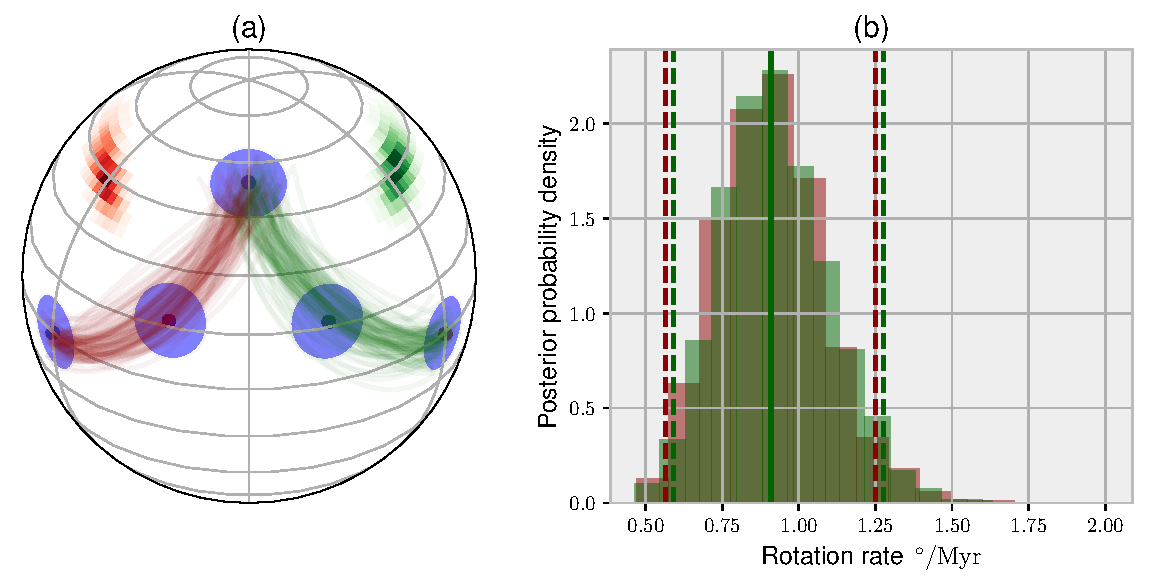
\includegraphics[width=0.9\textwidth]{figures/synthetic/two_euler_poles.pdf}
\caption{Inversion for two successive paleomagnetic Euler poles. (a) Five paleomagnetic poles are generated, beginning with a pole at $0^\circ$N, $60^\circ$W. The first Euler pole is located at $41^\circ$N, $60^\circ$W, and rotates at $6.5^\circ$/Myr for 20 Myr. The second Euler pole is located at $41^\circ$N, $60^\circ$W, and rotates at the same speed and for the same duration. The red and green distributions show the location of the first and second Euler poles (respectively) recovered by the MCMC inversion. The the red and green lines are a sampling of the synthetic APW paths generated by the inversion. (b) Posterior probability density for the rotation rates of the Euler poles recovered by the inversion.}
\label{fig:two_euler_poles}
\end{figure*}
\subsection{Incorporating age uncertainty}
\begin{figure*}
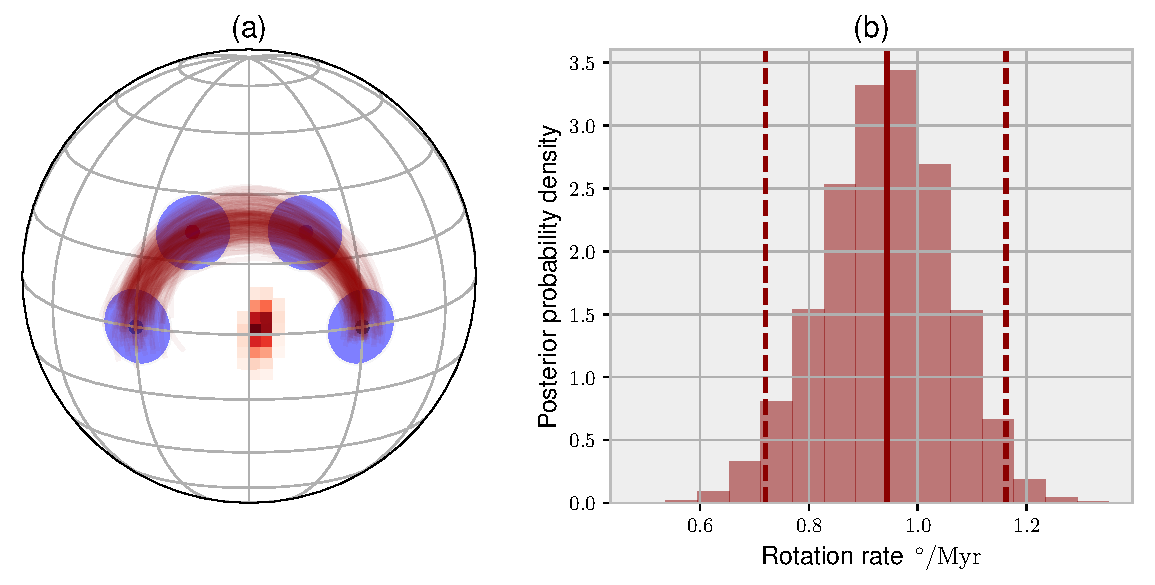
\includegraphics[width=0.9\textwidth]{figures/synthetic/age_uncertainty.pdf}
\caption{Inversion for two successive paleomagnetic Euler poles. (a) Five paleomagnetic poles are generated, beginning with a pole at $0^\circ$N, $60^\circ$W. The first Euler pole is located at $41^\circ$N, $60^\circ$W, and rotates at $6.5^\circ$/Myr for 20 Myr. The second Euler pole is located at $41^\circ$N, $60^\circ$W, and rotates at the same speed and for the same duration. The red and green distributions show the location of the first and second Euler poles (respectively) recovered by the MCMC inversion. The the red and green lines are a sampling of the synthetic APW paths generated by the inversion. (b) Posterior probability density for the rotation rates of the Euler poles recovered by the inversion.}
\label{fig:age_uncertainty}
\end{figure*}
\begin{figure*}
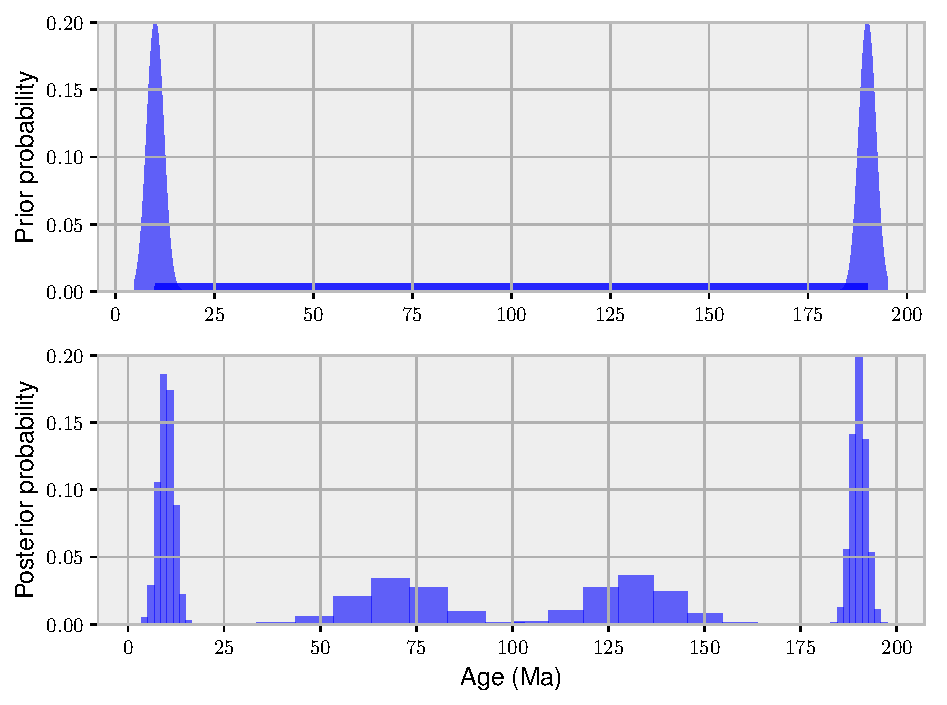
\includegraphics[width=0.9\textwidth]{figures/synthetic/age_uncertainty_samples.pdf}
\caption{Inversion for two successive paleomagnetic Euler poles. (a) Five paleomagnetic poles are generated, beginning with a pole at $0^\circ$N, $60^\circ$W. The first Euler pole is located at $41^\circ$N, $60^\circ$W, and rotates at $6.5^\circ$/Myr for 20 Myr. The second Euler pole is located at $41^\circ$N, $60^\circ$W, and rotates at the same speed and for the same duration. The red and green distributions show the location of the first and second Euler poles (respectively) recovered by the MCMC inversion. The the red and green lines are a sampling of the synthetic APW paths generated by the inversion. (b) Posterior probability density for the rotation rates of the Euler poles recovered by the inversion.}
\label{fig:age_uncertainty_samples}
\end{figure*}

\section{Application to Cenozoic Australian APW path}
\label{sec:australia}
\clearpage
\begin{figure*}
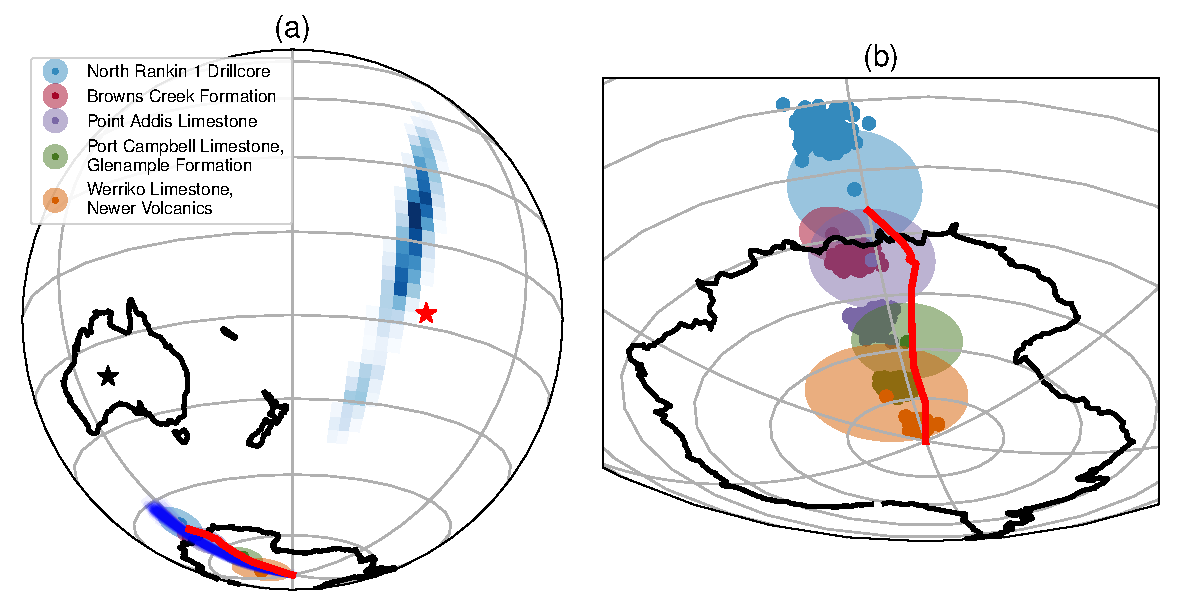
\includegraphics[width=0.9\textwidth]{figures/australia/australia_paths_1.pdf}
\caption{}
\label{fig:australia_paths_1}
\end{figure*}
\begin{figure*}
\includegraphics[width=0.9\textwidth]{figures/australia/australia_latitude_1.pdf}
\caption{}
\label{fig:australia_latitude_1}
\end{figure*}
\begin{figure*}
\includegraphics[width=0.9\textwidth]{figures/australia/australia_ages_1.pdf}
\caption{}
\label{fig:australia_ages_1}
\end{figure*}
\begin{figure*}
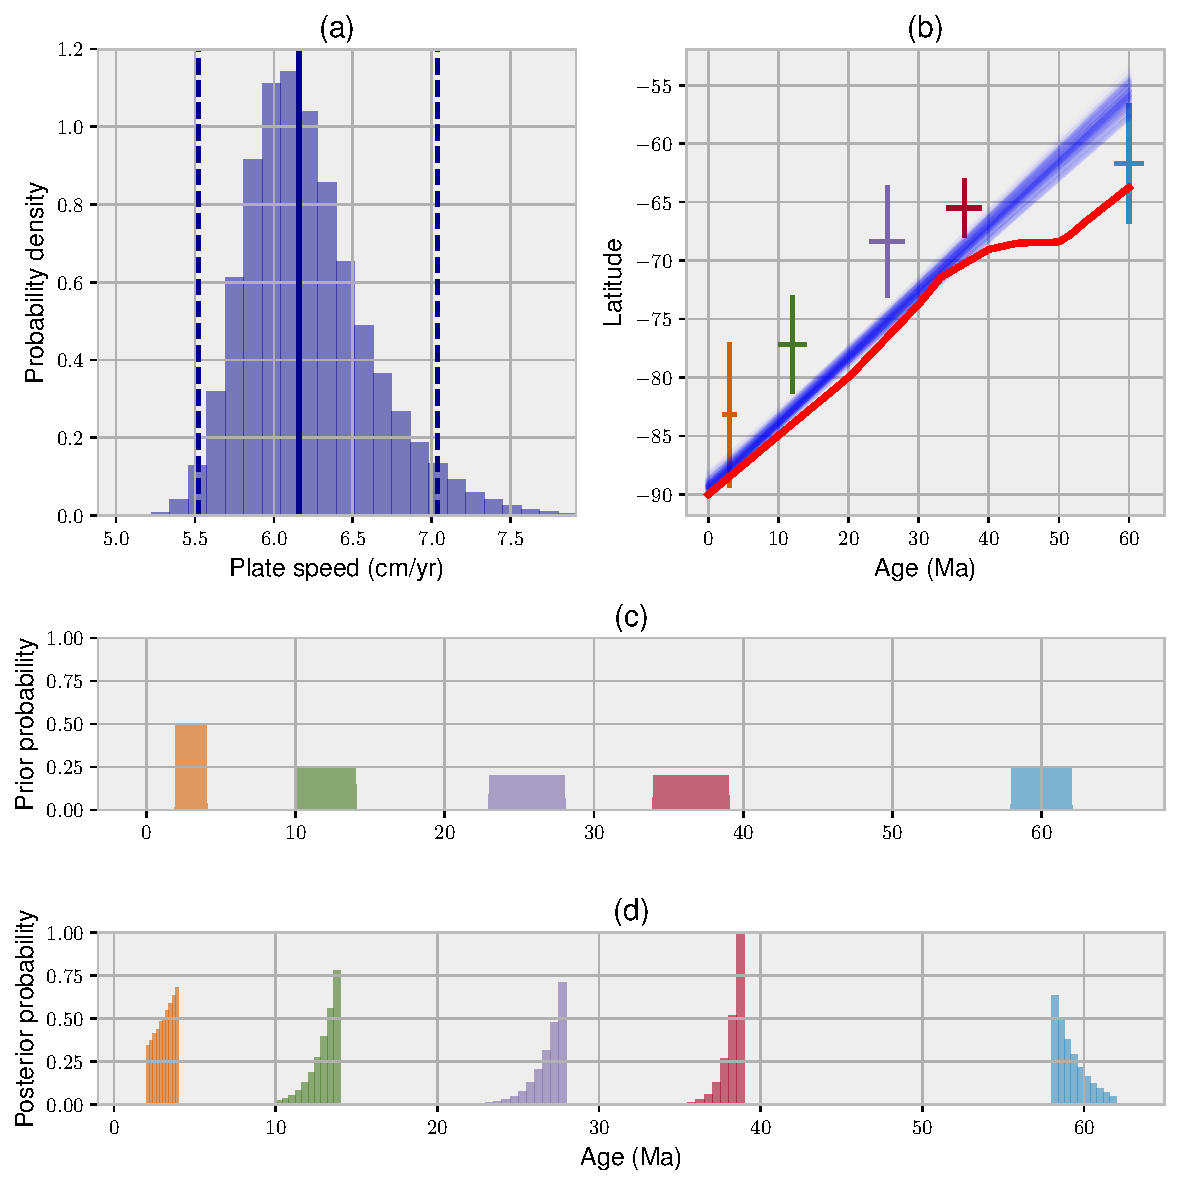
\includegraphics[width=0.9\textwidth]{figures/australia/australia_speeds_1.pdf}
\caption{}
\label{fig:australia_speeds_1}
\end{figure*}
\begin{figure*}
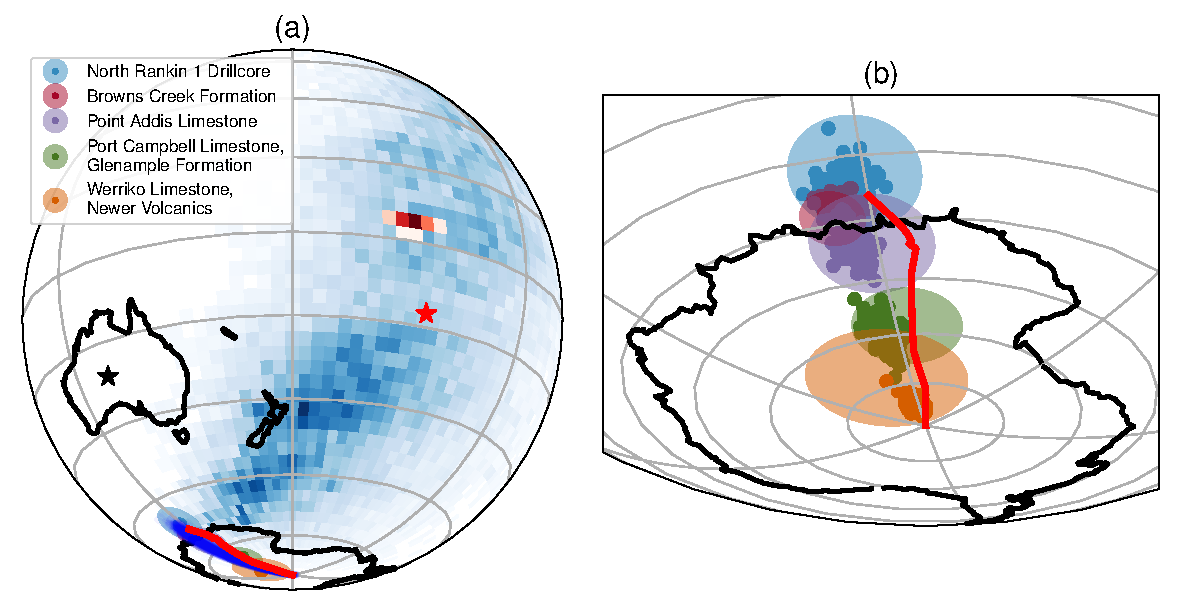
\includegraphics[width=0.9\textwidth]{figures/australia/australia_paths_2.pdf}
\caption{}
\label{fig:australia_paths_2}
\end{figure*}
\begin{figure*}
\includegraphics[width=0.9\textwidth]{figures/australia/australia_ages_2.pdf}
\caption{}
\label{fig:australia_ages_2}
\end{figure*}
\begin{figure*}
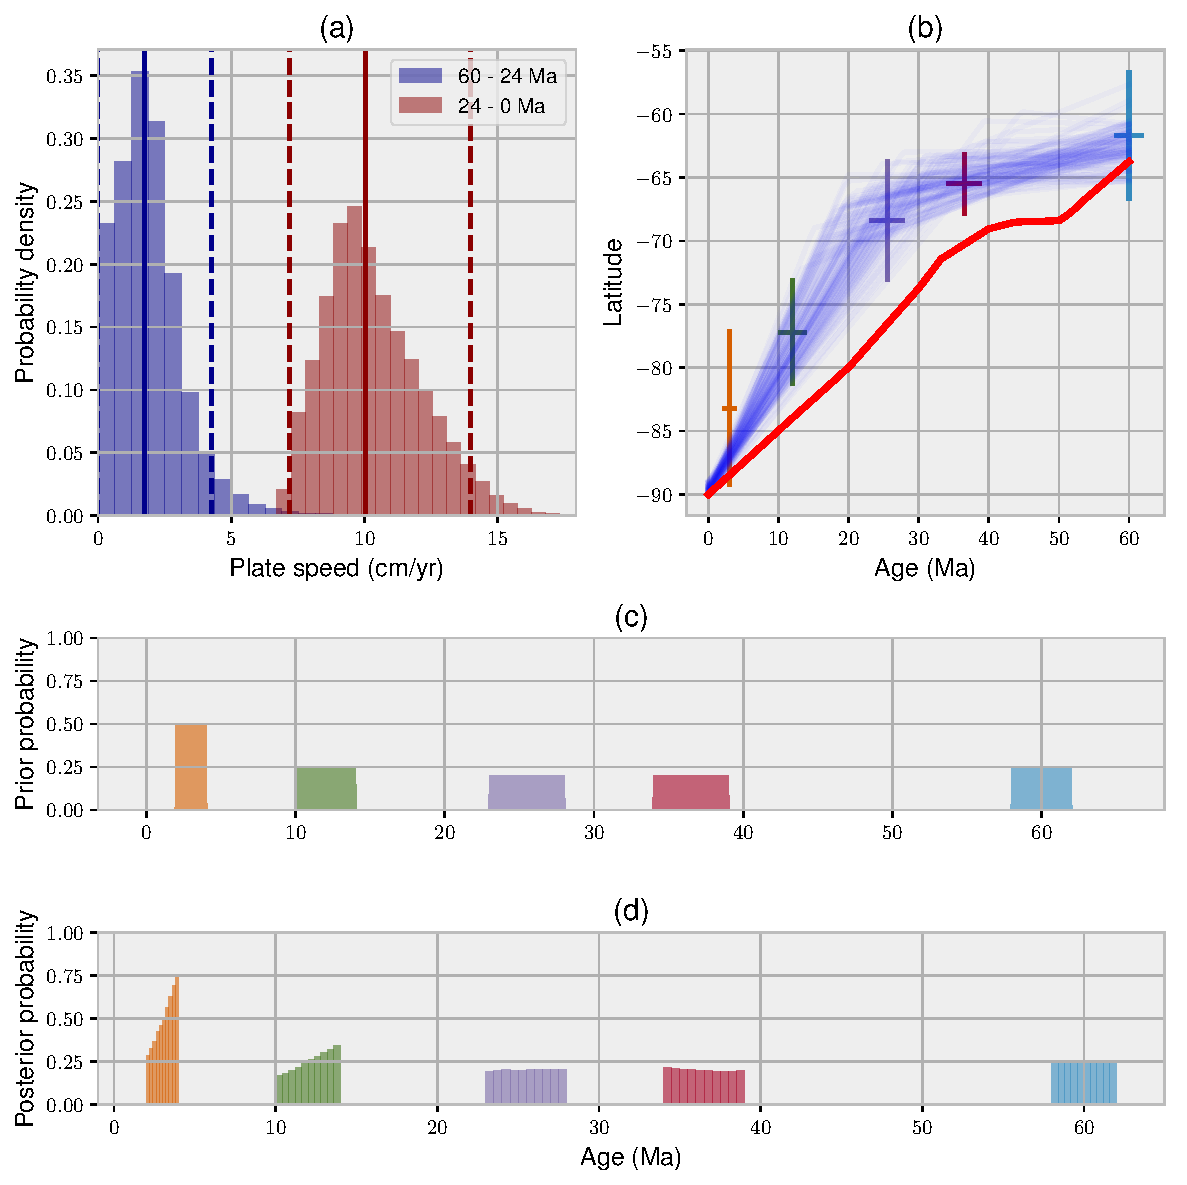
\includegraphics[width=0.9\textwidth]{figures/australia/australia_speeds_2.pdf}
\caption{}
\label{fig:australia_speeds_2}
\end{figure*}
\begin{figure*}
\includegraphics[width=0.9\textwidth]{figures/australia/australia_latitude_2.pdf}
\caption{}
\label{fig:australia_latitude_2}
\end{figure*}


\section{Application to the Keweenawan province}
\label{sec:keweenawan}
\subsection{Geologic context}
\citet{swanson2009no}
\subsection{Inversion for paleomagnetic Euler poles}
\clearpage
\begin{figure*}
\includegraphics[width=0.9\textwidth]{figures/keweenawan/keweenawan_paths_1.pdf}
\caption{}
\label{fig:keweenawan_paths_1}
\end{figure*}
\begin{figure*}
\includegraphics[width=0.9\textwidth]{figures/keweenawan/keweenawan_ages_1.pdf}
\caption{}
\label{fig:keweenawan_ages_1}
\end{figure*}
\begin{figure*}
\includegraphics[width=0.9\textwidth]{figures/keweenawan/keweenawan_speeds_1.pdf}
\caption{}
\label{fig:keweenawan_speeds_1}
\end{figure*}
\begin{figure*}
\includegraphics[width=0.9\textwidth]{figures/keweenawan/keweenawan_paths_2.pdf}
\caption{}
\label{fig:keweenawan_paths_2}
\end{figure*}
\begin{figure*}
\includegraphics[width=0.9\textwidth]{figures/keweenawan/keweenawan_ages_2.pdf}
\caption{}
\label{fig:keweenawan_ages_2}
\end{figure*}
\begin{figure*}
\includegraphics[width=0.9\textwidth]{figures/keweenawan/keweenawan_speeds_2.pdf}
\caption{}
\label{fig:keweenawan_speeds_2}
\end{figure*}
\begin{figure*}
\includegraphics[width=0.9\textwidth]{figures/keweenawan/keweenawan_paths_3.pdf}
\caption{}
\label{fig:keweenawan_paths_3}
\end{figure*}
\begin{figure*}
\includegraphics[width=0.9\textwidth]{figures/keweenawan/keweenawan_ages_3.pdf}
\caption{}
\label{fig:keweenawan_ages_3}
\end{figure*}
\begin{figure*}
\includegraphics[width=0.9\textwidth]{figures/keweenawan/keweenawan_speeds_3.pdf}
\caption{}
\label{fig:keweenawan_speeds_3}
\end{figure*}
\subsection{Plate speeds for Mesoproterozoic Laurentia}

\section{Conclusions}
\label{sec:conclusions}



%% The Appendices part is started with the command \appendix;
%% appendix sections are then done as normal sections
%% \appendix

%% \section{}
%% \label{}

%% If you have bibdatabase file and want bibtex to generate the
%% bibitems, please use
%%
\bibliographystyle{elsarticle-harv} 
\bibliography{bayesian_plate_reconstruction}

%% else use the following coding to input the bibitems directly in the
%% TeX file.

\end{document}

\endinput
%%
%% End of file `elsarticle-template-harv.tex'.
